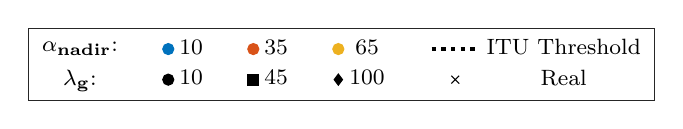
\begin{tikzpicture}
\definecolor{mycolor1}{rgb}{0.00000,0.44700,0.74100}%
\definecolor{mycolor2}{rgb}{0.85000,0.32500,0.09800}%
\definecolor{mycolor3}{rgb}{0.92900,0.69400,0.12500}%
%
\begin{axis}[%
width=0,
height=0,
at={(0,0)},
xmin=0,
xmax=0,
xtick={},
ymin=0,
ymax=0,
ytick={},
scale only axis,
axis background/.style={fill=white},
legend style={font=\footnotesize,legend cell align=center, align=center, draw=white!15!black,at={(0,0)},anchor=south west, /tikz/every even column/.append style={column sep = 0.5cm}},
legend columns = 5
]
\addlegendimage{empty legend};
\addlegendentry{$\mathbf{\alpha_{nadir}}$:}

\addlegendimage{scatter,only marks, mark=*, draw=mycolor1, fill=mycolor1};
\addlegendentry{\ang{10}}

\addlegendimage{scatter,only marks, mark=*,draw=mycolor2, fill=mycolor2};
\addlegendentry{\ang{35}}

\addlegendimage{scatter,only marks, mark=*, draw=mycolor3, fill=mycolor3};
\addlegendentry{\ang{65}}

\addlegendimage{color=black, dotted, line width=1.5pt};
\addlegendentry{ITU Threshold}

\addlegendimage{empty legend};
\addlegendentry{$\mathbf{\lambda_g}$:}

\addlegendimage{scatter,only marks, mark=*,draw=black, fill=black};
\addlegendentry{10}

\addlegendimage{scatter,only marks, mark=square*,draw=black, fill=black};
\addlegendentry{45}

\addlegendimage{scatter, only marks, mark=diamond*,draw=black, fill=black};
\addlegendentry{100}

\addlegendimage{scatter, only marks, mark=x,draw=black, fill=black};
\addlegendentry{Real}
\end{axis}
\end{tikzpicture}%

